\documentclass[12pt,a4paper]{article}
\usepackage{calc}% http://ctan.org/pkg/calc
\usepackage[
  letterpaper,%
  textheight={47\baselineskip+\topskip},%
  textwidth={\paperwidth-126pt},%
  footskip=75pt,%
  marginparwidth=0pt,%
  top={\topskip+0.75in}]{geometry}% http://ctan.org/pkg/geometry
\usepackage{fancyhdr}% http://ctan.org/pkg/fancyhdr

\usepackage{graphicx}
%\usepackage{subcaption}

\usepackage{hyperref}
\usepackage{amsmath}
\usepackage{color}

\definecolor{orange}{rgb}{1,0.5,0}

\newcommand{\kpar}{k_{||}}
\newcommand{\kperp}{k_\perp}
\newcommand{\bvec}{\mathbf{b}}
\newcommand{\deriv}[2]{\frac{\partial #1}{\partial #2}}

\pagestyle{fancy}
%\fancyhead{}
\fancyfoot{}% Clear header & footer
%\fancyhead[L]{Electrostatic Ohm's law}% Set centered header
%\fancyhead[R]{ 22$^{nd}$ March 2014 }
\fancyfoot[C]{\thepage}% Set centered footer
\renewcommand{\headrulewidth}{0.5pt}% Add header rule

% Titling
\title{ Two-phase flow model }% Your title
\author{ Ben Dudson }% Your author
\date{ 14$^{th}$ March 2017 }% Your date
\makeatletter
% Definition of proc.cls' \maketitle:
\def\@maketitle{% 
  \vbox to 1.25in{%
    \vskip 0.5em
    {\large \begin{tabular}[t]{ll}
        Title: & \@title \\
        Author: & \@author \\
        Date: & \@date \\
        Project: &
      \end{tabular}\par}
    \vfil}\noindent\hrulefill
    \vskip 2em}
\makeatother
\begin{document}
\maketitle % Produce title
\thispagestyle{fancy}% Override titling page style with fancy

\section{Model equations}

Equations for two immiscible incompressible fluids in 2D is solved using the vorticity formulation. The fluid velocity $\mathbf{u}$ is calculated using $\mathbf{u} = \nabla\times\mathbf{\psi}$, where in 2D only only one component of the stream function $\psi$ is needed. All code, inputs and analysis scripts used here are available at \url{https://github.com/bendudson/two-phase-flow}.

\subsection{Fluid interface tracking}

A Volume of Fluid (VOF) approach is used to track the interface between the two phases. A colour field $c$ is $0$ in one fluid, and $1$ in the other, transitioning between $0$ and $1$ at the boundary between them. The density $\rho$ and kinematic viscosity $\nu$ are given by
\begin{eqnarray}
\rho &=& \left(1-c\right)\rho_0 + c \rho_1 \\
\nu &=& \left(1-c\right)\nu_0 + c \nu_1 \\
\end{eqnarray}
The colour moves with the flow velocity $\mathbf{u}$:
\begin{equation}
\frac{\partial c}{\partial t} + \mathbf{u}\cdot\nabla c = 0
\end{equation}

This advection equation is solved using the following algorithm:
\begin{enumerate}
\item The stream function $\psi$ is interpolated onto cell corners, then derivatives taken along cell edges to calculate the flow
velocity through the cell faces.
\item A $1^{st}$-order upwinding algorithm is used to advect
  the field $c$ through cell faces.
\item In order to control the diffusion which would smear out
  the sharp boundary over time, a regularised anti-diffusion
  term is added, which acts to steepen the boundary between the
  fluids\footnote{K.K.So, X.Y.Hu, N.A.Adams J.Comp.Phys. 230 (2011) 5155-5177}. 
\end{enumerate}

\subsection{Momentum and vorticity}

Starting from the momentum equation:

\begin{equation}
\frac{\partial}{\partial t}\left(\rho \mathbf{u}\right) + \mathbf{u}\cdot\nabla\left(\rho\mathbf{u}\right) = -\nabla p - g\mathbf{e}_x + \rho\nu\nabla^2\mathbf{u} - \mathbf{F}_s
\end{equation}
take the $y$ component of the curl of this equation, to get
the vorticity in 2D ($x-z$).

The surface tension force per unit area of surface is
\begin{equation}
\mathbf{F}_A = \sigma\kappa\left(c\right)\mathbf{n}
\end{equation}
where $\sigma$ is a scalar coefficient of surface tension,
in Newtons per meter; $\kappa$ is the surface curvature (units 1/m); $\mathbf{n}$ is the unit vector normal to the surface.
This is represented using the Continuum Surface Force (CSF) formulation\footnote{J.U.Brackbill, D.B.Kothe, C.Zemach J.Comp.Phys 100, 335-354 (1992)} as a force per unit volume, given by:
\begin{equation}
\mathbf{F}_s = \sigma\kappa\left(c\right)\nabla c
\end{equation}
When integrated over a surface, $\nabla c$ gives $\left[c\right]$, which transitions from 0 to 1 across a surface, so recovers the force per unit area given above. 
The curvature $\kappa$ is related to the surface normal
\begin{equation}
\kappa = \nabla\cdot\left(\mathbf{n}\right)
\end{equation}
The surface normal can be approximated using the $c$ field:
\begin{equation}
\mathbf{n} = \nabla c / \left|\nabla c\right|
\end{equation}

Taking the curl of the surface force, the surface force term can be written 
as a Poisson bracket:
\begin{eqnarray}
\mathbf{e}_y\cdot\nabla\times \mathbf{F}_s &=& \mathbf{e}_y\cdot\nabla\left(\sigma\kappa\right)\times\nabla c \\
&=& -\mathbf{e}_y\times\nabla\left(\sigma\kappa\right)\cdot\nabla c \\
&=& -\left[\sigma\kappa, c\right]
\end{eqnarray}

Finally this gives the equation for the vorticity $\omega$:
\begin{equation}
\frac{\partial\omega}{\partial t} = -\left[\psi, \omega\right] - g\frac{\partial\rho}{\partial z} + \nu\nabla^2\omega - \left[\sigma\kappa, c\right]
\end{equation}

In this model the Poisson brackets are implemented using Arakawa's $2^{nd}$-order advection scheme.

\subsection{Calculation of curvature}
\label{sec:curvature}

Two methods for calculating the curvature $\kappa$ are implemented: A finite difference method and the Height Function method. 

The finite difference (FD) method uses a smoothed function of $c$, and calculates $\kappa = \nabla\cdot\mathbf{n}$ using finite differences\footnote{}.

The Height Function (HF) method is a $2^{nd}$-order scheme which integrates the function $c$ and then takes finite differences of those integrals\footnote{M.Sussman J.Comp.Phys. 187 (2003) 110-136}.
\section{Tests}

\subsection{Stationary bubble}

A standard test of two-phase fluid models is to test the
magnitude of parasitic (non-physical) flows around a stationary bubble. These arise from the calculation of curvature in VOF type schemes.
\begin{figure}[h]
\centering
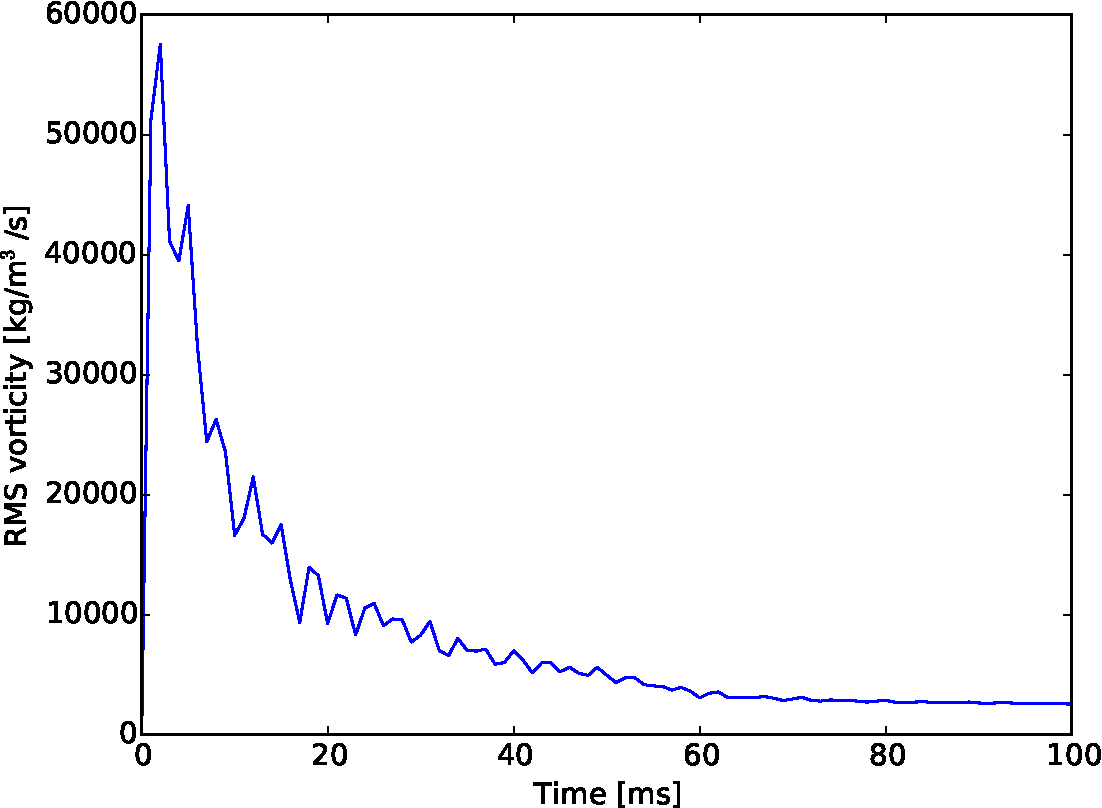
\includegraphics[width=0.45\textwidth]{bubble_vorticity.pdf}
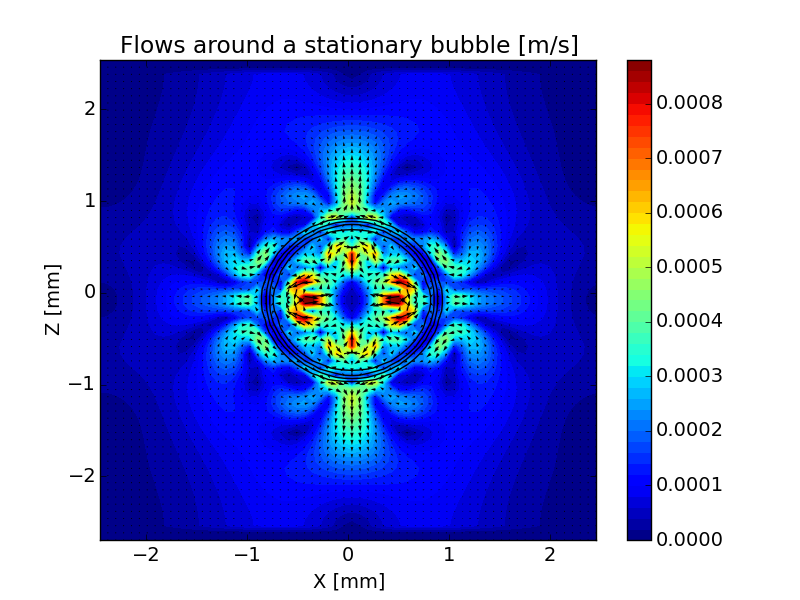
\includegraphics[width=0.45\textwidth]{bubble_flows.png}
\caption{Simulation of a stationary bubble of radius $\sim 1$mm. {\bf Left}: Evolution of the average (Root-Mean-Square) vorticity in the domain as a function of time. {\bf Right}: Final state showing flow magnitude (colours), direction (arrows), and the boundary of the bubble (black contours).}
\label{fig:bubble}
\end{figure}
Figure~\ref{fig:bubble} shows the evolution and final state of
a circular bubble. The two fluids have the same density $\rho=1000$kg/m$^3$ and kinematic viscosity $\nu=10^{-6}$m$^2$/s (approximately water). The surface tension is $\sigma=72$mN/m, similar to that for water-air interfaces. The curvature is calculated using the Finite Difference method. 

The vorticity initially increases and the width of the interface region grows. After around $60$ms a steady state is reached, with parasitic flows of the order of $1$mm/s.

\subsection{Capillary wave dispersion}

A sinusoidal perturbation of an interface between two fluids is simulated, based on simulations in [Denner 2017]\footnote{F.Denner et al. Computers and Fluids 143 (2017) 59-72}. Both fluids have the same density $\rho=1$kg/m$^3$ and kinematic viscosity $\nu = 1.6394\times 10^{−3}$m$^2$/s. The surface tension between the two fluids is $\sigma=0.25\pi^{-3}$N/m. The domain is $\lambda$ in width ($z$ direction here), and $3\lambda$ in height ($x$ direction). Results for wavelengths $\lambda=1$m and $\lambda=0.1$m are shown in figure~\ref{fig:capillary}.
\begin{figure}[h]
\centering
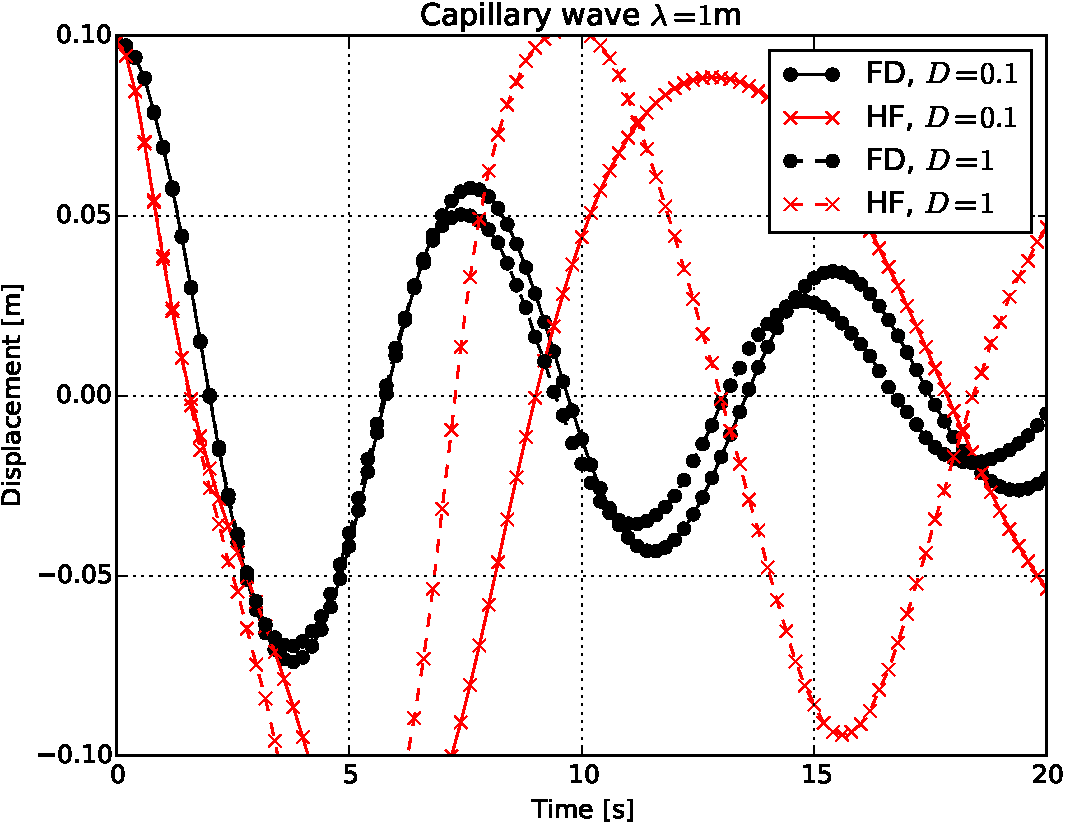
\includegraphics[width=0.45\textwidth]{capillary_2.pdf}
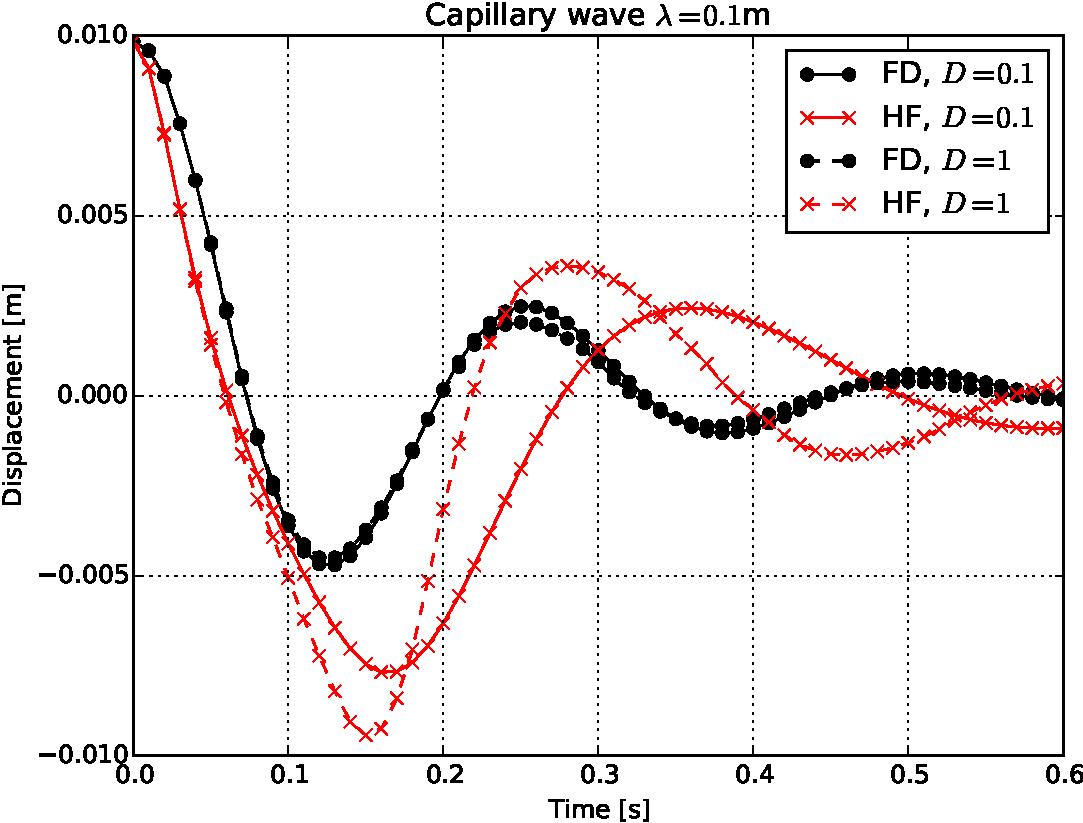
\includegraphics[width=0.45\textwidth]{capillary_1.pdf}
\caption{Evolution of the amplitude of a standing capillary wave, for comparison with figure 2 of [Denner 2017]}
\label{fig:capillary}
\end{figure}
This indicates that whilst the Finite Difference calculation of curvature gives good agreement, the Height Function method does not. Sharpening the interface by increasing the anti-diffusion $D$ improves the result.


\end{document}
